\section{Grafiken}

\subsection{Verschiedene Möglichkeiten}

Nun werden Grafiken eingefügt auf verschiedenste Weise.\\
Wie in der Abbildung \cref{fig:test_plot_1} zu sehen ist.

\begin{figure}[!ht]
	\centering
	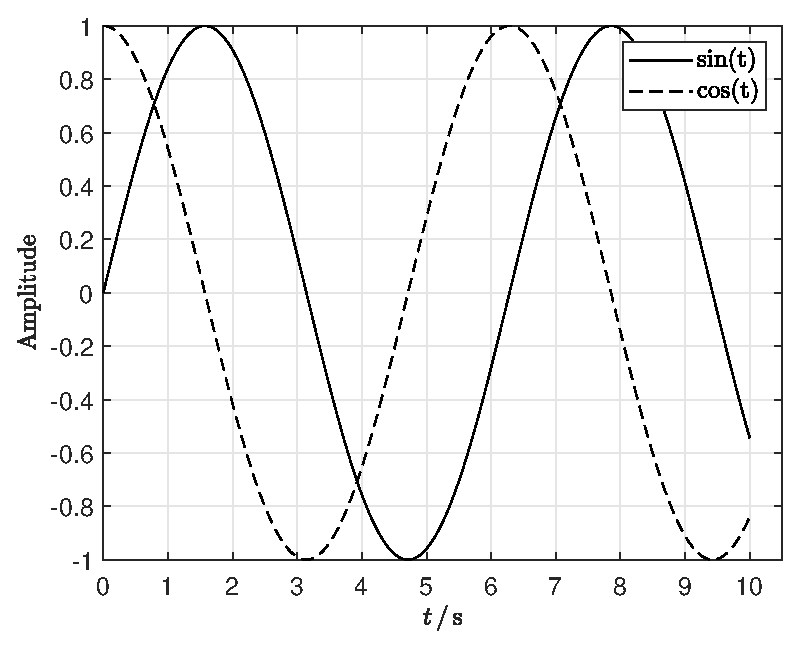
\includegraphics[width=0.6\textwidth]{Test_plot_1.eps}
	\caption[60\,\% der Textbreite]{Sinus- und Cosinus-Verlauf über die Zeit dargestellt.\cite{Sensoren}}
	\label{fig:test_plot_1}
\end{figure}


\clearpage
Die nächsten zwei Abbildungen (\cref{fig:subhouse21} und \cref{fig:subhouse22}) zeigen jeweils eine Möglichkeit zwei Grafiken nebeneinander einzufügen.\cite{Sensoren}
\begin{enumerate}
	\item Bei der Ausrichtung stehen der Möglichkeiten zur Auswahl: c (für Center) t (für Top) und b (für Bottom)
	\item Mit diesem folgenden Befehl kann das Bild skaliert werden \glqq\textit{keepaspectratio}\grqq{} und nach einem Anführungszeichen sollte immer ein Leerzeichen eingefügt werden mit einem Backslash, oder mit zwei geschwungenen Klammern.
\end{enumerate}

\clearpage
\begin{figure}[!ht]
	\begin{subfigure}[b]{.48\textwidth}
		\centering
		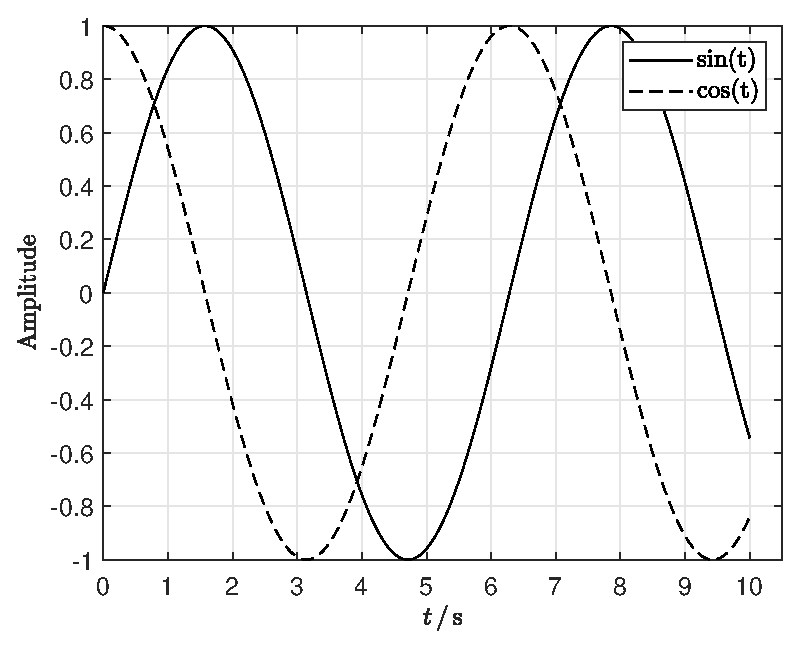
\includegraphics[width=0.95\textwidth]{Test_plot_1.eps}
		\caption{erster Affe}
		\label{fig:subhouse21}
	\end{subfigure}
	\hfil
	\begin{subfigure}[b]{.48\textwidth}
		\centering
		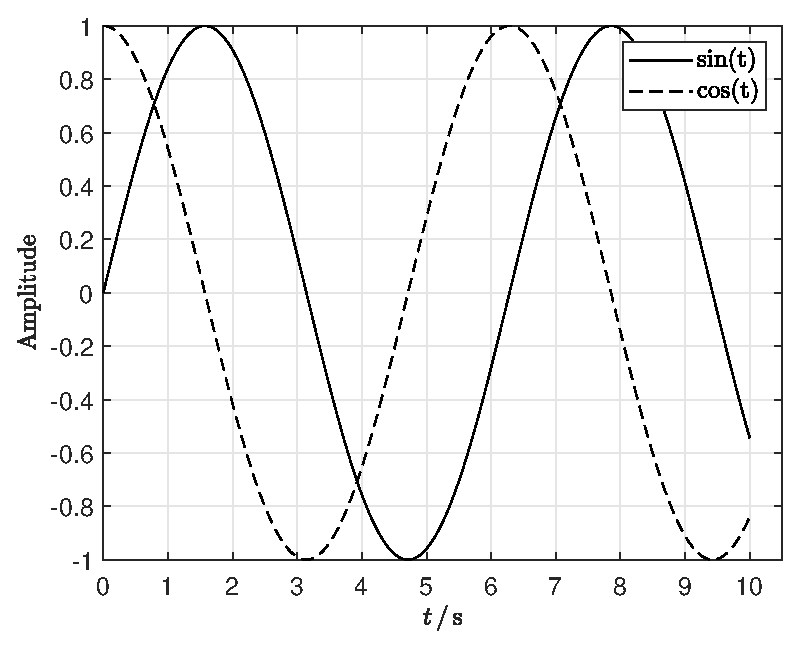
\includegraphics[width=0.95\textwidth]{Test_plot_1.eps}
		\caption{zweiter Affe}
		\label{fig:subhouse22}
	\end{subfigure}
	\caption[zwei Pferde]{Die Nebenstehenden Bilder sollten nach diesen Schema eingefügt werden. (Steht im Loborleitfaden)}    
	\label{fig:Doppelbild}
\end{figure}

\subsection{Bild und nebenbei eine Tabelle}
\begin{figure}[!ht]
	\begin{subfigure}[b]{.48\textwidth}
		\centering
		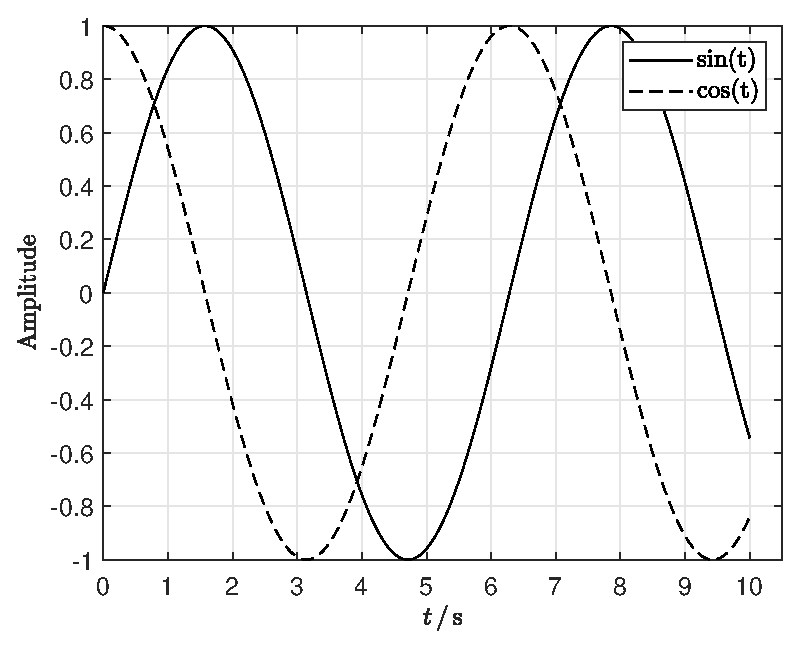
\includegraphics[width=0.95\textwidth]{Test_plot_1.eps}
		\caption{erster Affe}
		\label{fig:subhouse23}
	\end{subfigure}
	\hfil
	\begin{subfigure}[b]{.48\textwidth}
		\centering
		\resizebox{0.95\textwidth}{!}{
			\begin{tabular}{*{3}{c}}
				\hline
				Beschreibung & Abkürzung & Größe \\
				\hline
				Statische Verstärkung & $K$ & $0.71$\\
				Zeitkonstante 1 & $\tau_1$ & $0.24$\,\si{\second}\\
				Zeitkonstante 2 & $\tau_2$ & $0.68$\,\si{\second}\\
			\end{tabular}
		}
		\caption{zweiter Affe}
		\label{tab:subhouse123}
	\end{subfigure}
	\caption[Zwei Schweine]{Zwei Affen}
	\label{fig:subhouses2}
\end{figure}

So und jetzt ist genug mit den Grafiken, weiteres werden Tabellen erstellt bevor zu den mathematischen Formeln gewechselt wird. 
\clearpage

\section{Tabellen}


Verschieden bsp. Tabellen werden

\begin{table}[htp]
	\renewcommand{\arraystretch}{1.2} %% Abstand zwischen den Zeilen wird größer
	\centering
	\caption[Vorgegebene Größen]{Vorgegebene Größen}
	\label{tab: Vorgegebene Größen}
	\footnotesize
	%\resizebox{.6\textwidth}{!}{
		\begin{tabular}{*{3}{c}}
			\toprule
			Beschreibung & Abkürzung & Größe \\
			\midrule
			Versorgungsspannung & $U_b$ & $20$\,\si{\volt}\\
			Eingangsspannung & $U_{ein}$ & $\pm0,5$\,\si{\volt}\\
			Ausgangsspannung & $U_{aus}$ & $\pm5$\,\si{\volt}\\
			Untere Grenzfrequenz & $f_{gu}$ & $100$\,\si{\hertz}\\
			Obere Grenzfrequenz & $f_{go}$ & $10$\,\si{\kilo\hertz}\\
			Eingangswiderstand & $R_{ein}$ & $10$\,\si{\kilo\ohm}\\
			Lastwiderstand & $R_{aus}$ & $10$\,\si{\kilo\ohm}\\
			\bottomrule
		\end{tabular}
		%}    
\end{table}



\begin{table}[htp]
	\centering
	\caption[Vorgegebene Größen\_1]{Vorgegebene Größen\_1}
	\label{tab: Vorgegebene Größen_1}
	\footnotesize
	%\resizebox{.5\textwidth}{!}{
		\begin{tabular}{l l r}
			\toprule
			Beschreibung & Abkürzung & Größe \\
			\midrule
			Versorgungsspannung & $U_b$ & $20$\,\si{\volt}\\
			Eingangsspannung & $U_{ein}$ & $\pm0,5$\,\si{\volt}\\
			Ausgangsspannung & $U_{aus}$ & $\pm5$\,\si{\volt}\\
			Untere Grenzfrequenz & $f_{gu}$ & $100$\,\si{\hertz}\\
			Obere Grenzfrequenz & $f_{go}$ & $10$\,\si{\kilo\hertz}\\
			Eingangswiderstand & $R_{ein}$ & $10$\,\si{\kilo\ohm}\\
			Lastwiderstand & $R_{aus}$ & $10$\,\si{\kilo\ohm}\\
			\bottomrule
		\end{tabular}
		%}
\end{table}

\section{Formeln}

Diese folgende Formel \ref{eqn:omsches Gesetz} wird unter Verwendung auch mit dem Symbolverzeichnis verknüpft. 


\begin{equation}
	{U}={R}\cdot{I}
	\Rightarrow
	{I}=\frac{U}{R}
	\label{eqn:omsches Gesetz}
\end{equation} 

Gleichung \cref{eqn:Gleichung} über mehrere Zeilen
\begin{eqnarray}
	\Delta L&=&\int\limits_0^L(1-\cos\varphi)\,dx\approx\int\limits_0^L[1-(1-\varphi^2/2)]\,dx=\frac{1}{2}\int\limits_0^Lw'^2\,dx=\nonumber\\
	&=&\frac{B^2\lambda^2}{2}\int\limits_0^L\cos^2\lambda x\,dx=\frac{B^2\lambda^2}{2}\left[\frac{\lambda x-\sin\lambda x\cos\lambda x}{2\lambda}\right]_0^L\approx\frac{B^2\lambda^2L}{4}
	\label{eqn:Gleichung}
\end{eqnarray}

\begin{align}
	\begin{split}
		&\dot{\Vec{z}} = \boldsymbol{A}\Vec{z}+ \boldsymbol{B}v = \begin{bmatrix} 0 & 1 \\ 0 & 0 \end{bmatrix} \Vec{z}+\begin{bmatrix} 0 \\ 1\end{bmatrix} v \\
		&y = \boldsymbol{C}\Vec{z} = \begin{bmatrix}1 & 0\end{bmatrix} \Vec{z} \\
	\end{split}
	\label{eqn:statelin}
\end{align}



